\chapter{基于循环神经网络的脑电P300检测方法}

对于深度学习中的另一种网络——循环神经网络, 目前很少有方法对非侵入式信号进行处理, 但我们注意到循环神经网络可以很好地利用时间维度相关性对时间序列进行建模, 而其中的长短时间记忆方法可以很好地避免传统循环神经网络训练难以收敛的问题。 因此, 本文中设计了LSTMP300Net, 采用长短时间记忆方法对EEG信号建模 , 使其能够更好地拟合信号在P300检测任务上的信号特性。 最后在实验中, 我们比较了ConvP300Net和LSTMP300Net, 结果表示LSTMP300Net比ConvP300Net效果强2.8\%。


\section{循环神经网络}

人类可以很快地识别节奏模式序列,即那些有时间间隔的子模式。此外,鼓手等演奏者也能根据运动命令生成有精确时间节奏的节奏序列。这促使人们研究人工系统,去分离或产生通过事件间时间间隔长度传递信息的模式。

Deep Neural Network(DNN)通常在较难的learning问题上能够达到比较好的效果。 在实际问题中有很多是时序信号,如语音识别, 连续(即字符无分割的)手写识别, 蛋白质分析,股市预测等。 虽然这些问题无论是否有监督,都可以交给CNN或者DNN处理并达到较好效果\cite{abdel2014convolutional,lecun1995convolutional,ciresan2011convolutional,lecun1994word,lauer2007trainable,baldi1996hybrid,zhu2014stock},但是并不能完全利用上信号的时序性,而循环神经网络(recurrent neural network)可以利用神经元循环传递实现时序信号的分析。

一个循环神经网络是一个结构中带反馈连接的神经网络, 它可以学习并处理时序序列问题, 而传统的机器学习算法由于没有考虑时间方面相关性可能并不善于解决这类问题。 之前对于这种时序信号的处理方法是一些基于可学习可适应的方法, 如隐马尔可夫模型\cite{eddy1996hidden}, 前向网络等, 但是在计算能力和物理意义上RNN都比这些方法能力强。 而且事件在时域上的信息很大程度上反映了时序任务的重要信息, 如运动控制和节奏检测。 隐马尔可夫模型往往忽视这一信息, 而循环神经网络( Recurrent Neural Network, RNNs)可以学习并应用这个信息。 隐马尔可夫模型(HMM)能够成功地应用在语音识别是因为这种方法不需要针对特定语速生成不同模型。 但是像节奏检测, 音乐处理, 和其他连续文本处理任务就都需要精确的时间测量。 虽然HMM可以通过给每个时间间隔单独创建一个内部状态来解决有限个时间间隔的问题, 但是这样既麻烦又低效, 并且没有用到HMM的非线性时序伸展不变性。

事实上, 尽管隐马尔克夫模型等传统时序信号处理算法可以在离散状态空间对数据进行分析, 但RNNs在根本上上适用于所有的序列学习任务, 因为它们具有图灵能力\cite{siegelmann1995computational}。 典型的RNN学习算法在一个潜在抗噪算法的通用空间中进行梯度下降\cite{pearlmutter1995gradient}, 这个通用算法采用分布式, 用连续值表示的内部状态来将实值的输入序列映射为实值输出序列。 所以循环神经网络在识别由时间距离定义的模式上更有效。 混合HMM的RNN方法\cite{bengio1995input}可能能够结合两种方法的优点,但就我们所知, 这种方法从未被用到准确的事件计时的问题。



\subsection{循环神经网络网络结构}

下面我们来看RNN的结构:
RNN包含一些用带权连接的单元,每个单元有一个在时间$t$更新的激活函数$y(t), t=1,2,…$。对单元$i$的激活$y^{i}$通过计算网络中与$i$的相连输入$net^{l}(t)$得到:
\begin{equation}
	net^{l}(t) = \sum_m{w_{im}y^m(t-1)}
\end{equation}
而后通过一个可导函数$f$将$net^{l}(t)$进行”压平”($f$比如我们之前提到的sigmoid, tanh, 或Relu函数):
\begin{equation}
	y^{i}(t) = f(net^i(t))
\end{equation}
其中网络的输入是随时间变化的序列,对于传统的RNN回归问题或者序列分类问题(如手写体识别),输出也是随时间变化的序列。而对于纯分类问题,输出只是一个标量。为了方便讲述传统RNN的方法,我们在这里使用输入输出都是时间序列来描述。

对有监督的RNN而言,当采用平方和误差作为loss时,我们将每个单元的损失计为与其输入与真实输入之差,而全局损失函数为所有样本损失的平方和,即t时刻的总误差为:
\begin{equation}
 \begin{array}{lr}
E(t) = \frac{1}{2}\sum_i{{e_i(t)}^2}\\
e_i(t) := Y^i(t) –y^k(t)
 \end{array}
\end{equation}

整个序列的误差为每一时刻的误差$E(t)$之和。


和CNN类似,RNN可以用梯度下降进行网络参数更新,即对于每个权重$w_{im}$,有
$\partial w_{im} = -\alpha \frac{\partial E(t)}{\partial w_{im}}$,其中$\alpha$为学习率。这种方法也是标准RNN的更新方法backpropagation through time (BPTT)方法,通过带入可得t时刻i单元的误差信息为

\begin{equation}
\partial e_i(t) = f_i’(net_i(t))\sum_j{w_{ji}e_j(t+1)}
\end{equation}

然而在1990年,Schmidhuber的学生Hochreiter提出RNN在理论上很好,但是不好训练,误差会以指数增长或者消失\cite{williams1995gradient},原因是BPTT, real-time recurrent learning(RTRL)\cite{williams1989learning},这类基于梯度下降的方法都有一个问题,如果计算权重更新后的q步,则如公式\ref{Eq:rnn_bptt}所示,t时刻与t-q的更新误差之比与$w_{lv}$有关,

\begin{equation}\label{Eq:rnn_bptt}
	\frac{\partial e_v(t-q)}{\partial e_u(t)} = 
	\left\{
	\begin{array}{lr}
		f'v(net_v(t-1))w_{uv}, q=1\\
		f'v(net_v(t-q))\sum_{l=1}^n{\frac{\partial e_l(t-q+l)}{\partial e_u(t)}w_{lv}}, q>1
	\end{array}
	\right.
\end{equation}

将上式$q>1$的情况展开,用$l_t$表示t时刻的该节点,$l_q = v, l_0 = u$,可得:
\begin{equation}
 \frac{\partial e_v(t-q)}{\partial e_u(t)} = \sum_{l1=1}^n ... \sum_{m=1}^q{\prod_{m=1}^q{f_{l_m}'(net_{l_m}(t-m))w_{l_ml_{m-1}}}}
\end{equation}

其中$\prod_{m=1}^q{f_{l_m}'(net_{l_m}(t-m))w_{l_ml_{m-1}}}$决定了总的传回误差。所以如果$|{f_{l_m}'(net_{l_m}(t-m))w_{l_ml_{m-1}}}|>1.0$,,则最大的乘积随q指数增长,就会使学习过程不稳定;相反地,如果$|{f_{l_m}'(net_{l_m}(t-m))w_{l_ml_{m-1}}}|<1.0$,则最大的乘积随q指数下降以至消失, 在有限时间内无法学到有效网络参数, 即在传统RNN中,反传的误差要不就收缩太快,要不就爆发超出界限。 这也被称为长时间延时问题(long time lag problem),使得RNN的应用一度局限在短时间序列。 事实上误差会随着网络层数而指数型衰减或爆发,因此很难训练, 而且不能处理长时间延时事件。 针对这个问题, Hochereiter提出了一种新型的RNN——长短时间记忆Long Short-Term Memory \cite{hochreiter1997long} (LSTM)网络。 LSTM网络有效克服了这一问题,我们将在下一节中予以介绍,关于RNN,更多优化方法请参考Bengio在\cite{bengio2013advances}中的综述。








\section{长段时间记忆网络}
\subsection{LSTM的网络结构与训练}
长段时间记忆(LSTM)网络中的基本单元是包含一个或多个存储单元(memory cell)和所有cell共享的三个自适应乘法门的存储块(memory block)。每个存储单元都在其中心有一个自连接单元,我们称之为“恒误差旋转木马”( Constant Error Carousel, CEC ),它本质上是一个无参数的线性单元。通过无限循环地进行激活和误差信号传递,CEC可以在延长的时间段内提供短期存储。Gers et al在LSTM中安置了忘记门 \cite{gers2000learning}。输入,忘记和输出门可以通过训练分别进行学习,即学会将什么信息存入,怎样保存,什么时候读出。
 

LSTM的体系结构允许LSTM容忍输入的事件之间有很长的时间延时(1000步及以上);而传统RNN用代价更高的更新算法,比如BPTT \cite{williams1990efficient},RTRL \cite{robinson1987utility,williams1989learning},或它们的组合\cite{schmidhuber1992fixed,williams1995gradient},都无法学习超过10个时间延时的序列\cite{hochreiter1991untersuchungen,bengio1994learning,hochreiter1997long, gers2000learning,hochreiter2001gradient}.

比如,一些我们以前任务需要用LSTM网络对发生于50个离散时间间隔之前的事件予以响应,而不受发生于之前49个时间间隔的事件的影响。就在关键时刻之前,如果有一个有用的“标记”输入通知网络,其下一步的行动将是至关重要的。因此,网络没有必要学习度量50个步骤的时间间隔;它只需要学会保存这50步的相关信息,而后一旦观察到这个标记就用这段信息即可。

但是如果没有这样的标记呢?如果网络本身需要学习测量并在内部表示这段特定任务的间隔内信息,或生成由特定时间间隔分割的序列模式,就要求在长时间连续输入流中保持网络的时间精确行和鲁棒性。显然,这样的任务通常不能由基于共同时间窗口的方法解决的,因为它们的泛化能力受时间窗口大小的限制。不幸的是,这意味着我们不能用标准基准进行测试和计时,因为就我们所知,目前没有任何其他网络学会将15个时间滞后推广到45个等。因此,我们不得不以创建一组新的比较任务。那就将用到LSTM了。

因为长短期记忆方法已被证明在长时间滞后任务上比其他RNN的方法强,而且其体系结构与人脑对信息的处理方式很类似,考虑到这种方式可能可以更好地模拟大脑皮层信号激发方式,所以我们研究该方法。LSTM通过内部细胞到多门的“窥孔连接”,在没有任何段式训练样本的情况下可以很好的区分50个和49个时间间隔的spike序列。在没有外部复位和监督学习的情况下,LSTM的变种也能学习生成时间精确的稳定spike流和其他非线性周期模式。这使得LSTM在需要的精确测量或生成有时间间隔的任务上很有效。


\subsection{LSTM相关工作}

在应用方面, LSTM在语音识别、连续手写识别、音乐合成、生物医药方面都有相关应用。 LSTM RNN是著名语音识别数据库TIMIT的benchmark (Graves et al, ICASSP 2013), Nicole等人用大量数据在LSTM网络进行RNN的retraining\cite{beringer2005classifying},这是无法在HMM中实现的。 google用LSTM RNN来改善大规模语音识别\cite{sak2014long}。在类似问题上,\cite{sutskever2014sequence}将LSTM应用在机器翻译问题,实现了sequences to sequence学习。 连续(即字符无分割的)手写识别方面,  Connectionist Temporal Classification(CTC)\cite{graves2012connectionist}训练的RNN(CTC-LSTM)\cite{bluche2014a2ia},在2009年跑得结果赢了很多手写识别竞赛的冠军\cite{graves2006connectionist}。 音乐合成方面, RNN的变种RNN-RBM可以无监督地形成简单的钢琴旋律\cite{boulanger2012modeling}。 通过用音乐集训练LSTM网络,网络就可以无监督地生成有特定样式的旋律与和弦的音乐样本, 而前向网络和传统RNN都无法学习出和弦音\cite{eck2002first}。 生物医药方面, 在RNN中还可以实现无分割的蛋白质分析\cite{hochreiter2007fast}, 其本质和无分割的手写体识别同理。





\subsection{LSTM的网络结构}
LSTM通过设置恒定的传递误差来解决上面提到的长时间延时问题。 在基本LSTM单元中, LSTM引入了一个自连接线性单元, 称作误差旋转木马(error carousel), 恒定的传递误差中设定权重$w$恒等于1, $f$为线性函数, 目的是这各部分只起到传递误差的作用,而将学习参数作用于其他权重。

LSTM以memory block作为基本单元,其中包含一个至多个memory cell,典型的LSTMmemory cell如图\ref{Fig:lstm_simple}所示:
核心有一个线性单元(或者称作线性神经元,如图橘黄色所示), 这是个线性单元, 在任意给定时间, 该单元将其所有输入通过加权连接求和。 它的自循环连接权重固定为1(即与左边紫色圆点之间的半圆连接权重固定为1), 这样通过确保训练信号或者误差在被传递的时候不会消失(vanish)克服了原先RNN的一个主要问题:vanish(参考3.2节)。 而且这个核心神经元为线性让LSTM实现了可以识别多达1000步之前的模式。 


\begin{figure}[htb]
  \centering
  % Requires \usepackage{graphicx}
  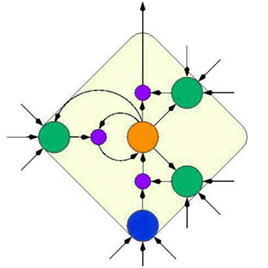
\includegraphics{Pictures/LSTM/lstm_simple.png}\\
  \caption{LSTM模型Memory block结构}\label{Fig:lstm_simple}
\end{figure}

在CEC核心周围是非线性可适应神经元, 用来学习非线性神经动作。 图中蓝色神经元用来表示输入, 三个绿色神经元分别表示三个门(左边的是忘记门,右下角为输入门,右上角为输出门),这些门通过学习来使核心线性神经元不受无关事件和误差信号的干扰, 而又能通过有效信息更新网络参数,即门是否打开来决定信号的有效性。 最后, 紫色圆点用以表示乘积操作。 LSTM的学习算法是非常高效的,每个边权的计算复杂度不超过O(1)。


LSTM的应用中, 可以将多个memory cell进行组合, 如图\ref{Fig:lstm_mixture}所示混合模型。 其中有两个memory cell, 分别从输入和输入门接受输入, 每个cell将输出结果分别传给另一个memory cell的输入, 输入门, 输出门和忘记门。 但实际应用中,通常将一至多个memory cell组合成memory block, 共享输入, 输出, 忘记门的权重(而不共享输入的权重),这样可以减少自适应参数的数量, 同时使block内部各cell起到不同作用。 

\begin{figure}[htb]
  \centering
  % Requires \usepackage{graphicx}
  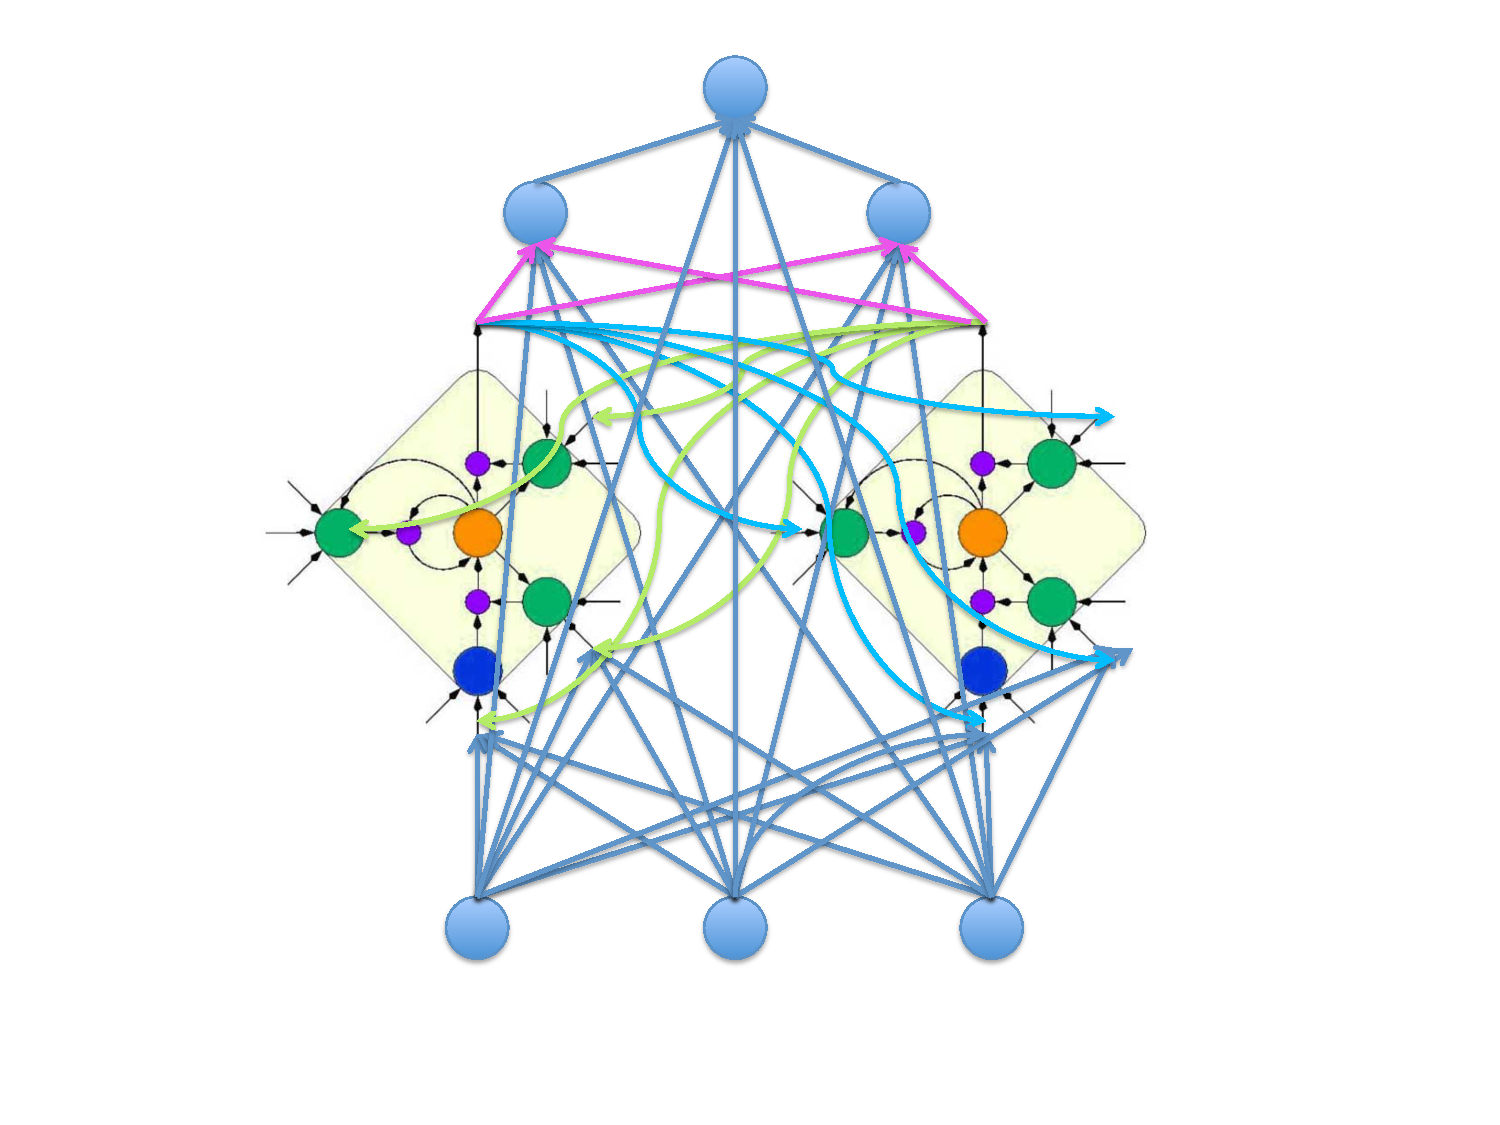
\includegraphics[scale = 0.5]{Pictures/LSTM/lstm_mixture_model.pdf}\\
  \caption{LSTM混合模型}\label{Fig:lstm_mixture}
\end{figure}

LSTM的发展过程经历了约10年: 1995至1997年,  Hochreiter 和 Schmidhuber 提出LSTM,包括cell,input gate, output gate的概念, 训练方法为Real time recurrent learning(RTRL)和BPTT, 只有cell的误差(梯度)被反传回来,其他循环连接都被截断了。 1999年,  Gers等人在LSTM中加入了forget gate. 这使得LSTM可以学习连续任务(如Reber grammar)。2000年, Gers 和 Schmidhuber 提出加入窥孔连接(peephole connections)。 这样可以使LSTM可以学习需要精确时间定位的任务。 所谓peephole connections,就是从LSTM中间的那个CEC但愿到各个门的连接。 2005年, Graves 和 Schmidhuber 提出完全用BPTT进行LSTM网络训练, 并给出了TIMIT数据集上的benchmark。





\section{LSTMP300Net进行P300检测}

在这一节中, 我们利用LSTM进行P300分类。 如第三章数据集介绍, 这里我们应用同样的P300波形进行P300检测。 

\subsection{网络结构}
在P300检测任务中, 我们设置LSTM的网络结构LSTMP300Net如图\ref{Fig:LSTMP300Net}所示。 共设有一个输入层, 一个输出层, 中间3个隐层。 其中, 三个隐层$LSTM_1$,$LSTM_2$,$LSTM_3$ 均为LSTM层, 分别有2, 3, 2个节点, 每个节点为一个memory block。 此外, 我们设置每个memory block中含有两个memory cell, 同一个block内的cell共享输入门, 输出门和忘记门, 这些门使得各cell可以在时间维度进行信息存储。 每个block将各cell的输出结果输入同层其他block和上一层。 其中, 每个block从输入, 输入门, 输出门, 忘记门接受输入。 


\begin{figure}[htb]
  \centering
  % Requires \usepackage{graphicx}
  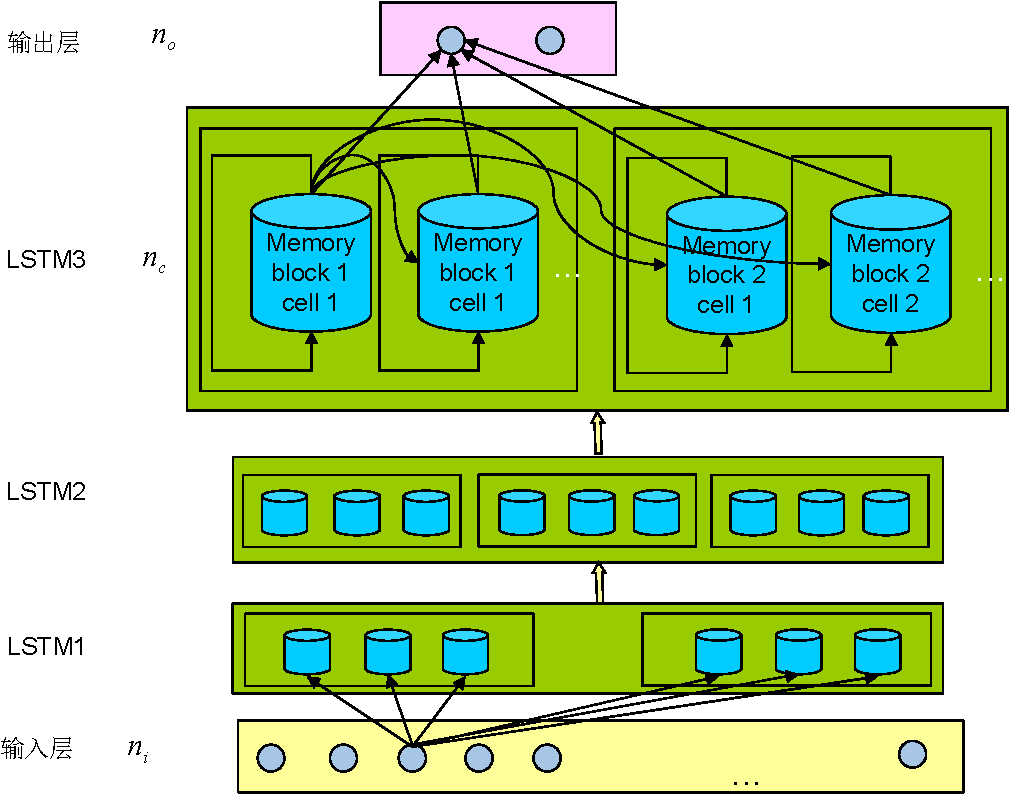
\includegraphics{Pictures/LSTM/LSTMP300Net-crop.pdf}\\
  \caption{LSTMP300Net网络模型}\label{Fig:LSTMP300Net}
\end{figure}


\subsection{网络训练}
在LSTMP300Net中, 我们选择交叉熵(crossEntropy)作为训练损失目标函数。 信息论中, 交叉熵用来度量复杂度, 如压缩问题中, 交叉熵表示平均需要几个bit来编码一个词。 用$p(x)$表示样本的真实分布, $q(x)$表示样本的估计分布, 则式\ref{Eq:ce_continuous}和\ref{Eq:ce_discrete}分别为连续数据和离散数据的信息熵表示。 

\begin{equation}\label{Eq:ce_continuous}
	H(p,q) = \int_x f(x)\log f(x)
\end{equation}

\begin{equation}\label{Eq:ce_discrete}
	H(p,q) = -\sum_x p(x)\log q(x)
\end{equation}

在机器学习问题中, 常用交叉熵定义损失函数, 用$p_i$表示样本的真实标号, $q_i$ 为当前模型对样本的估计标号, 即:
\begin{equation}
	H(p,q)=-\sum_i{p_i\log q_i}
\end{equation}
实际上, 逻辑回归方法中的损失函数就是所有样本交叉熵的平均值, 即
\begin{equation}
	L(w) = -\frac{1}{N}\sum_{i=1}^N {[y_i \log g(x_i)+(1-y_i)\log (1-g(x_i))]}
\end{equation}

LSTM网络中用最小化交叉熵代替最大似然估计。 在\cite{erdogmus2002error}中有相关证明, 最小化交叉熵和最小化$d(y, g(x))$是等价的, 其中$d(y, g(x))$表示样本真实标号和网络估计的标号距离。 这说明通过最小化交叉熵可以将LSTM网络输出收敛到目标标号分布。 在LSTM网络训练时, 我们采用backpropagation through time(BPTT)算法\cite{williams1990efficient}, 将时序LSTM网络在时间维展开成一个多层前向网络, 每个时间点作为前向网络的一层。
和前向神经网络相同, LSTM中每个隐层节点在t时刻的输出$o_j(t)=f(net_j(t))$, 不同的是, 每个时刻隐层节点输入的线性组合不仅要考虑上一层(即上一时刻)传来的输出$o_i(t-1)$, 还要考虑当前时刻的输入$x(t)$:
\begin{equation}
	net_j(t)=\sum_{i=1}^{l}x_i(t)w_{ij} + \sum_k{o_k(t-1)w_{kj}}
\end{equation}
其中$w_{ij}$表示节点i到j的权重, $l$为输入样本的维度, k为所有与j节点相连的节点的下标。 从隐层到输出层, 有
\begin{equation}
	y_k(t) = g(net_k(t))
\end{equation}
\begin{equation}
	net_k(t) = \sum_j o_j(t)w_{jk}
\end{equation}
其中, $g$函数为输出层的激励函数, $f$为隐层的激励函数, 我们在LSTM网络中要学习的是参数$v$和$w$, $w$和前向网络中的连接权重类似, $v$为隐层节点$t$时刻到$t+1$时刻的连接权重。 和传统误差反传算法类似, 我们在这里求取反传误差$\delta$, 然后根据$\delta$对LSTM网络中的权重参数进行优化。


\subsection{实验结果}

本实验中, 我们仍旧用上一章中的BCI竞赛数据做P300检测。 将15300个训练数据中的95\%作为训练数据, 剩余5\%作为验证数据, 采用18000个测试数据。 通过模型调整, LSTMP300Net在主体A和B上平均比ConvP300Net效果强2.80\%。


\subsubsection{交叉熵与分类错误率}

首先, 我们用当前LSTMP300Net在训练集上训练, 由于收敛较快, 所以我们只进行15次迭代。 最后分别选择验证集上分类准确率和交叉熵最小的一轮迭代作为试验结果。 如图\ref{Fig:LSTMP300Net_cross}和\ref{Fig:LSTMP300Net_class}分别为用LSTMP300Net做主体B的P300波形检测所得的交叉熵和分类错误率随迭代次数变化的曲线。 从图中可见, 在训练集和测试集上, 误差和交叉熵整体都呈降低趋势。 在第11轮迭代时, 分类误差几乎不变。 在实验结果中, 第10轮迭代在验证集上得到了最小交叉熵, 第12轮迭代时在验证集上得到了最小分类错误率。 此时, 测试集上得到的分类错误率分别为 15.59\% 和 15.57\%, 与ConvP300Net的P300波形检测结果相当。

 
\begin{figure}[htb]
  \centering
  % Requires \usepackage{graphicx}
  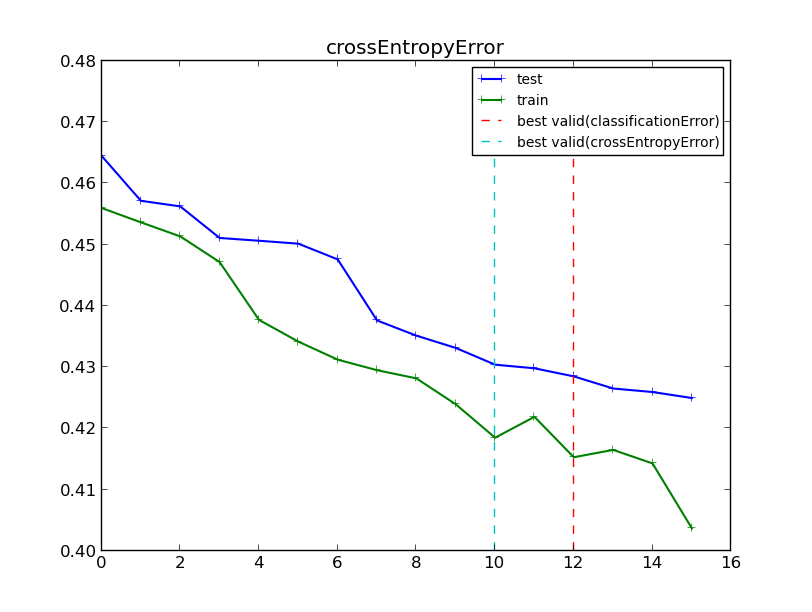
\includegraphics[scale=0.6]{Pictures/LSTM/crossentropy.png}\\
  \caption{LSTMP300Net交叉熵损失函数-迭代次数}\label{Fig:LSTMP300Net_cross}
\end{figure}


\begin{figure}[htb]
  \centering
  % Requires \usepackage{graphicx}
  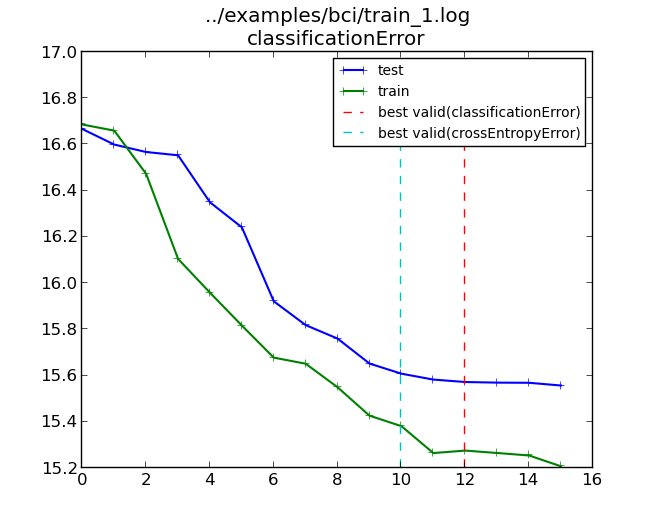
\includegraphics[scale=0.6]{Pictures/LSTM/classificationError.png}\\
  \caption{LSTMP300Net分类错误率-迭代次数}\label{Fig:LSTMP300Net_class}
\end{figure}

\subsubsection{模型变换}

基于当前模型, 我们在本节中做一些改进, 通过调整模型参数后进行训练, 查看P300波形检测效果是否有所改进。 这里我们用了3个LSTMP300Net的变种, LSTM1Cell, LSTM2Layer与LSTM1C2L。 这里,  LSTM1Cell与LSTMP300Net的层数相同,但每个记忆块(memory block)中只有1个cell, 这是为了化简模型, 并取消多cell共享门带来的不确定性; LSTM2Layer比LSTMP300Net少了LSTM3那一层, 因为层数过多模型不容易调整; LSTM1C2L结合了LSTM1Cell和LSTM2Layer, 只采用了LSTMP300Net中的前两层, 且每层中每个记忆块只用了1个cell。 这三个模型及ConvP300Net, LSTMP300Net在主体A, B中的P300检测结果如表\ref{Tab:LSTM_multi}所示。

\begin{table}[ht]
\centering
  \caption{实验人A —— P300 检测各卷积神经网络结果}
  \begin{tabular}{|c||c|c|c|c|c|c|c|c|}
  \hline
   & TP & TN & FP & FN & Reco.(\%) & Recall & Precision & F-value \\
  \hline\hline
	ConvP300 & 2216 & 11402 & 3598 & 784 & 75.656  & 0.739  & 0.381  & 0.503 \\
	\hline
	LSTMP300 & 2049&	11721&	3279&	951&	0.765& 	0.683& 	0.385& 	0.492  \\
	\hline
	LSTMCell1 & 2242 & 11419 & 3581 &	758&	0.759 & 0.747 &	0.385& 0.508\\
	\hline
	LSTM2Layer & 2231	&11486&	3514&	769&	0.762& 	0.744& 	0.388& 	0.510 \\
	\hline
	LSTM1C2L & 2254&	11907&	3093&	746&	0.787& 	0.751& 	0.422& 	0.540  \\
	\hline
  \end{tabular}
  \centering \label{tab:p300_cnn_A}
\end{table}


\begin{table}[ht]
\centering
  \caption{实验人B —— P300 检测各卷积神经网络结果}
  \begin{tabular}{|c||c|c|c|c|c|c|c|c|}
  \hline
   & TP & TN & FP & FN & Reco.(\%) & Recall & Precision & F-value \\
  \hline\hline
  	ConvP300 & 2537 & 12679 & 2321 & 463 & 84.533 & 0.846 & 0.522 & 0.646 \\
	LSTMP300 & 2512	&12847	&2153	&488	&0.853 &	0.837 &	0.538 &	0.655   \\
	\hline
	LSTMCell1 & 2546&	12680	&2320	&454	&0.846 &	0.849 &	0.523 &	0.647 \\
	\hline
	LSTM2Layer & 2552&	12692&	2308&448	&0.847 &	0.851 	&0.525& 	0.649  \\
	\hline
	LSTM1C2L & 2571	&12890&	2110&	429	&0.859 &	0.857 &	0.549 &	0.669 \\
  \hline
  \end{tabular}
  \centering \label{tab:p300_cnn_B}
\end{table}


从表中可见,LSTMP300Conv的简化模型——LSTM1C2L效果最佳, 在主体A,B上分别达到78.7\%和85.9\%的识别率, 平均超过ConvP300Net 2.80\%。